\documentclass[11pt]{beamer}
\usetheme{CambridgeUS}
\usepackage[utf8]{inputenc}
\usepackage{amsmath}
\usepackage{amsfonts}
\usepackage{amssymb}
\usepackage{graphicx}
\usepackage{pgfpages}
\usepackage{framed}
\usepackage{xcolor}
\usepackage[most]{tcolorbox}
\usepackage{soul}
\usepackage{empheq}

% The replacement character � (often displayed as a black rhombus with a white
% question mark) is a symbol found in the Unicode standard at code point U
% +FFFD in the Specials table. It is used to indicate problems when a system 
% is unable to render a stream of data to a correct symbol.[4] It is usually 
% seen when the data is invalid and does not match any character. For this 
% reason we map explicitly this character to a blanck space.
\DeclareUnicodeCharacter{FFFD}{ }

\newcommand*{\itemimg}[1]{%
  \raisebox{-.3\baselineskip}{%
    \includegraphics[
      height=\baselineskip,
      width=\baselineskip,
      keepaspectratio,
    ]{#1}%
  }%
}

\newtcbox{\mymath}[1][]{%
    nobeforeafter, math upper, tcbox raise base,
    enhanced, colframe=blue!30!black,
    colback=blue!10, boxrule=1pt,
    #1}

\newcommand{\highlight}[1]{%
  \colorbox{yellow!100}{$\displaystyle#1$}}

\author{Giovanni Della Lunga\\{\footnotesize giovanni.dellalunga@unibo.it}}
%\title{4.1 - Linear and Logistic Regression}
%\title{4.2 - Decision Trees}
\title{3.2 - Support Vector Machines}
%\title{6 - Text Vectorization}
%\title{7 - Classification for Text Analysis}
%\title{8 - Clustering for Text Similarity}
%\title{9 - Information Extraction}
\subtitle{} % (optional)
\setbeamercovered{transparent} 
\institute{Introduction to Machine Learning for Finance} 
\date{Bologna - February, 2022} 

\begin{document}

%\begin{frame}
%\includegraphics[width=\linewidth]{img/halloween-seminar-logo.PNG}
%\end{frame}

\begin{frame}
\titlepage
\end{frame}

\AtBeginSection[]
{
  %\begin{frame}<beamer>
  %\footnotesize	
  %\frametitle{Outline}
  %\begin{multicols}{2}
  %\tableofcontents[currentsection]
  %\end{multicols}	  
  %\normalsize
  %\end{frame}
  \begin{frame}
  \vfill
  \centering
  \begin{beamercolorbox}[sep=8pt,center,shadow=true,rounded=true]{title}  	\usebeamerfont{title}\insertsectionhead\par%
  \end{beamercolorbox}
  \vfill
  \end{frame}
}
\AtBeginSubsection{\frame{\subsectionpage}}

% INSERT HERE
\begin{frame}{Support Vector Machines}
	\begin{itemize}
		\item In this section we consider another popular category of supervised learning models known as \textbf{support vector machines};
		\item Like \textbf{decision trees}, SVMs can be used for either classification or for the prediction of a continuous variable;
		\item We first consider \textbf{linear classification} where a linear function of the feature values is used to separate observations and in particular we will focus on \textbf{binary classification} where the separation is  into only two categories;
	\end{itemize}
\end{frame}
%..................................................................
\begin{frame}{Linear Separation}
\begin{columns}[T] % align columns
\begin{column}{.48\textwidth}
        \begin{itemize}
		\item \textbf{Linearly Separable Data points}: Data points can be said to be linearly separable if a separating boundary/hyperplane can easily be drawn showing distinctively the different class groups. 
		\item Linear separable data points mostly require linear machine learning classifiers such as Logistic regression for example.
        \end{itemize}
\end{column}%
\hfill%
\begin{column}{.48\textwidth}
    %\fbox{
        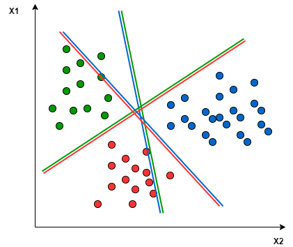
\includegraphics[width=\linewidth]{../5-pictures/chapter-4-4_pic_0.png}
    %}
\end{column}%
\end{columns}
\end{frame}
\begin{frame}{Linear Separation}
	\begin{center}
	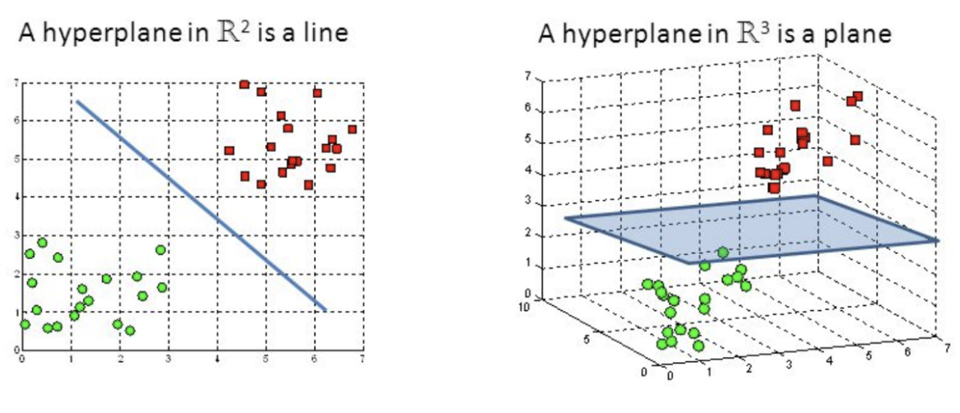
\includegraphics[scale=0.4]{../5-pictures/chapter-4-4_pic_1.png}
	\end{center}
\end{frame}
%..................................................................
\begin{frame}{Linear Separation }
	\begin{itemize}
		\item Binary classification can be viewed as the task of separating feature space into two halves;
		\item A simple situation is that in which we attempt to classify loans into good loans and defaulting loans;
	\end{itemize}
	\begin{center}
	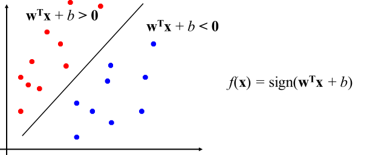
\includegraphics[scale=1]{../5-pictures/chapter-4-4_pic_2.png}
	\end{center}
\end{frame}
%..................................................................
\begin{frame}{Loans Classification Example}
	\begin{itemize}
		\item Consider two features: \textbf{credit score} and \textbf{income} of the borrower;
		\item We carry out an approximate scaling by subtracting 620 from the credit score (normalization);
		\item See Table 5.1 Hull
	\end{itemize}
	\begin{center}
	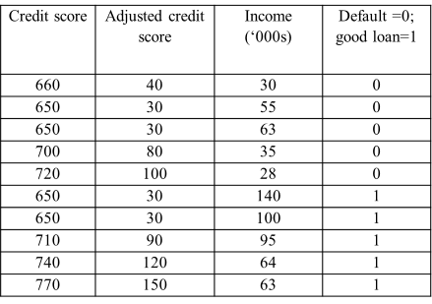
\includegraphics[scale=0.5]{../5-pictures/chapter-4-4_pic_3.png}
	\end{center}
\end{frame}
%..................................................................
\begin{frame}{Loans Classification Example}
	\begin{itemize}
		\item This is a \textbf{balanced data set} in that there are five good loans that defaulted;
		\item SVM does not work well for a seriously imbalanced data set and, if this is your condition, you need to use procedures to correct for this. 
	\end{itemize}
	\begin{center}
	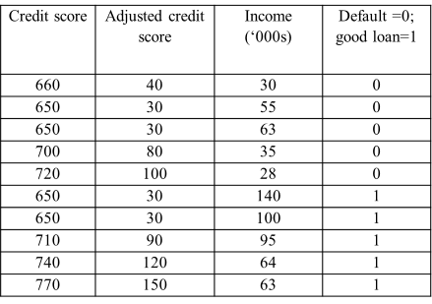
\includegraphics[scale=0.5]{../5-pictures/chapter-4-4_pic_4.png}
	\end{center}
\end{frame}
%..................................................................
\begin{frame}{Linear Separation}
	circles are defaulting loans, squares are good loans
	\begin{center}
	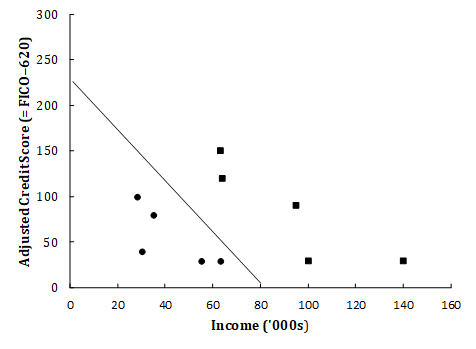
\includegraphics[scale=0.75]{../5-pictures/chapter-4-4_pic_5.png}
	\end{center}
\end{frame}
%..................................................................
\begin{frame}{Linear Separation}
	\begin{itemize}
		\item Which of the linear separators is optimal? 
	\end{itemize}
	\begin{center}
	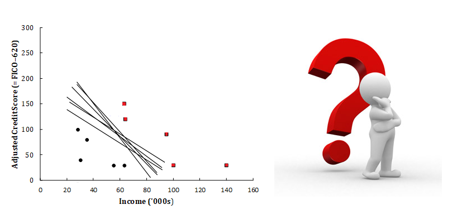
\includegraphics[scale=1]{../5-pictures/chapter-4-4_pic_6.png}
	\end{center}
\end{frame}
%..................................................................
\begin{frame}{SVM Approach}
	\begin{itemize}
		\item In the support vector machine (SVM) approach we find a pathway that separates the data into two classes as far as possible
		\item In the \textbf{hard margin} case perfect separation is possible (as in our example)
		\item The algorithm finds the widest path possible
		\item Data must be normalized. (We carry out approximate normalization by subtracting 620 from credit score)
		\item \highlight{\text{The support vectors are the observations at the edge of the pathway}}
	\end{itemize}
\end{frame}
%..................................................................
\begin{frame}{Example}
	Best pathway for example. Solid line would be used to distinguish good and bad loans
	\begin{center}
	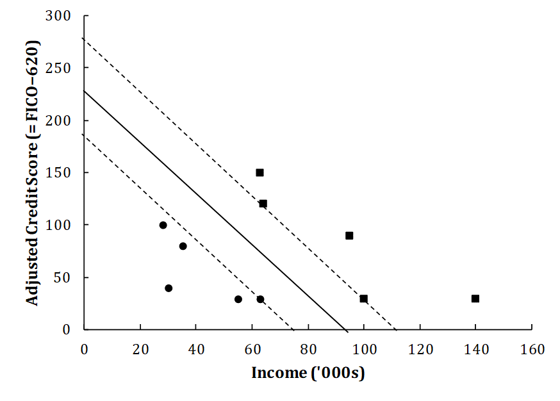
\includegraphics[scale=0.5]{../5-pictures/chapter-4-4_pic_7.png}
	\end{center}
\end{frame}
%..................................................................
\begin{frame}{SVM Approach}
	\begin{center}
	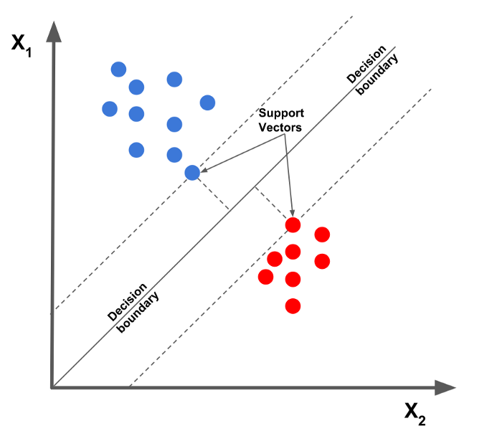
\includegraphics[scale=0.5]{../5-pictures/chapter-4-4_pic_8.png}
	\end{center}
\end{frame}
%..................................................................
\begin{frame}{SVM Approach: Notation}
	\begin{center}
	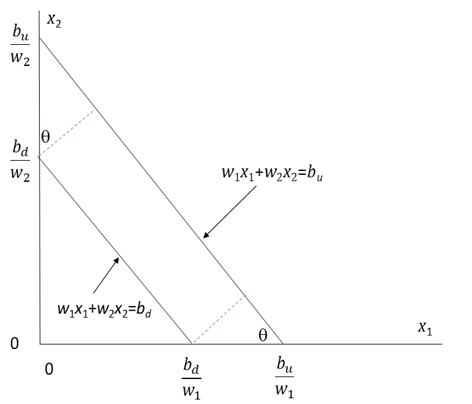
\includegraphics[scale=0.6]{../5-pictures/chapter-4-4_pic_9.png}
	\end{center}
\end{frame}
%..................................................................
\begin{frame}{The Math}
	\begin{center}
	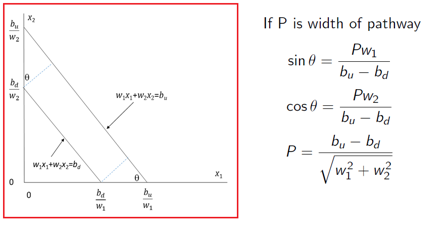
\includegraphics[scale=1]{../5-pictures/chapter-4-4_pic_10.png}
	\end{center}
\end{frame}
%..................................................................
\begin{frame}{The Math}
	\begin{itemize}
		\item We can scale $w_1$, $w_2$, $b_u$, and $b_d$  by the same constant without changing the model. 
		\item We can therefore set $b_u=b+1$ and $b_d=b-1$ so that the width of the pathway is $$P = \frac{2}{\sqrt{w_1^2+w_2^2}}$$
		\item In the \textbf{hard margin} case the algorithm minimizes $w_1^2+w_2^2$ subject to \textbf{perfect separation} being achieved
	\end{itemize}
\end{frame}
%..................................................................
\begin{frame}{The Math}
	\begin{itemize}
		\item For the example in table 5.1 we can set $x_1$ equal to income and $x_2$ equal to credit score;
		\item All good loans must be to the north-east of the pathway while all defaulting loans must be to the south west of the pathway;
		\item This means that, if a loan is good, the income and credit score must satisfy: $$w_1x_1 + w_2x_2 \ge b+1$$
		\item While if the loan defaults it must satisfy: $$ w_1x_1 + w_2x_2 \le b-1 $$
	\end{itemize}
\end{frame}
%..................................................................
\begin{frame}{Example}
	\begin{itemize}
		\item Specification of hard margin problem for our example
		\item In our example the task is to find $b$, $w_1$, and $w_2$ to minimize subject to
	\end{itemize}
	\begin{center}
	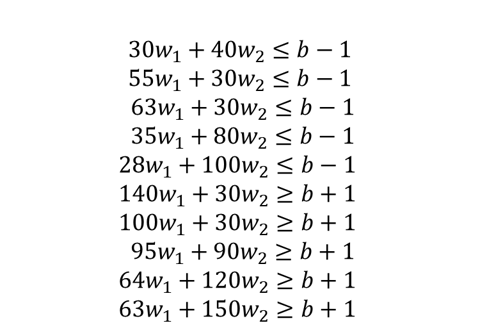
\includegraphics[scale=0.5]{../5-pictures/chapter-4-4_pic_11.png}
	\end{center}
\end{frame}
%..................................................................
\begin{frame}{The general hard margin problem}
	\begin{itemize}
		\item The objective function is $$\sqrt{w_1^2+w_2^2 + \dots + w_n^2}$$
		\item We minimize this for values of $w_i$ and $b$  subject to the condition that there are no violations, i.e.: $$\sum_i w_ix_i - b > 1 \quad \text{if loan good}$$ $$\sum_i w_ix_i - b < -1 \quad \text{if loan bad}$$
	\end{itemize}
\end{frame}
%..................................................................
\begin{frame}{Hard Margin Vs Soft Margin}
	\begin{center}
	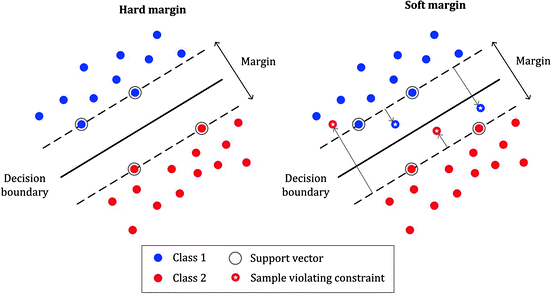
\includegraphics[scale=0.75]{../5-pictures/chapter-4-4_pic_12.png}
	\end{center}
\end{frame}
%..................................................................
\begin{frame}{The soft margin problem}
	\begin{itemize}
		\item We measure the violation of an observation as the extent to which the hard margin condition is violated
		\item we minimize $$C \cdot \text{sum of violations} + \sqrt{\sum_i w_i^2}$$
		\item Changing $C$  changes the trade-off between the width of the path and the violations
		\item As $C$ becomes smaller the pathway becomes wider with more violations
	\end{itemize}
\end{frame}
%..................................................................
\begin{frame}{Changed example: }
	\begin{center}
	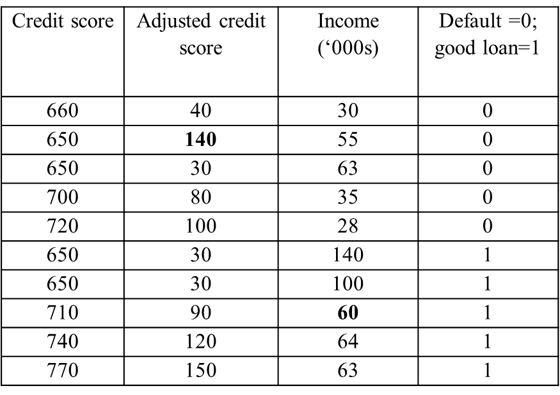
\includegraphics[scale=0.5]{../5-pictures/chapter-4-4_pic_13.png}
	\end{center}
\end{frame}
%..................................................................
\begin{frame}{Example}
	$C=0.001$ results
	\begin{center}
	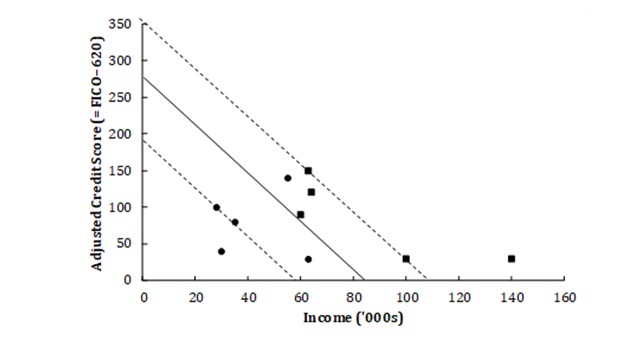
\includegraphics[scale=0.5]{../5-pictures/chapter-4-4_pic_14.png}
	\end{center}
\end{frame}
%..................................................................
\begin{frame}{Impact of C for Example}
	\begin{center}
	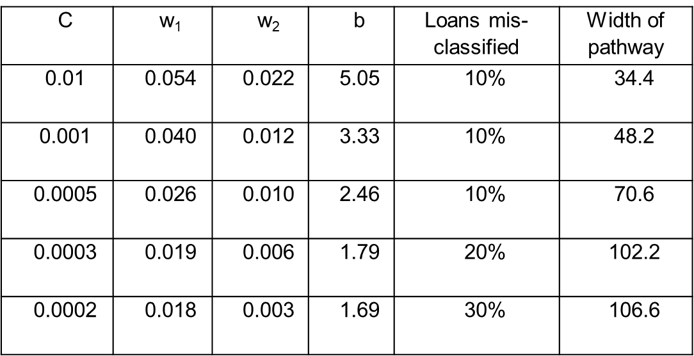
\includegraphics[scale=0.5]{../5-pictures/chapter-4-4_pic_15.png}
	\end{center}
\end{frame}
%..................................................................
\begin{frame}{Non Linear Separability}
	\begin{itemize}
		\item \textbf{Non-Linearly Separable data points}: This is the exact opposite of Linearly separable data points. 
		\item View the image below, notice that no matter how one tries to draw a straight line, some data points will one way or the other get misclassified. 
	\end{itemize}
	\begin{center}
	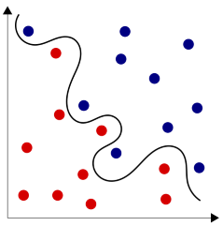
\includegraphics[scale=0.5]{../5-pictures/chapter-4-4_pic_16.png}
	\end{center}
\end{frame}
%..................................................................
\begin{frame}{Non-linear classification}
	\begin{itemize}
		\item The objective is to create new features so that the boundary becomes linear
		\item Suppose there is a single feature (age?) and we find the low and high values of the feature tend to give one outcome while intermediate values give another outcome
		\item We could form a new feature as $(\nu-m)^2$ where $\nu$ is the feature value and $m$ is its mean
	\end{itemize}
\end{frame}
%..................................................................
\begin{frame}{The Kernel Trick}
	\begin{center}
	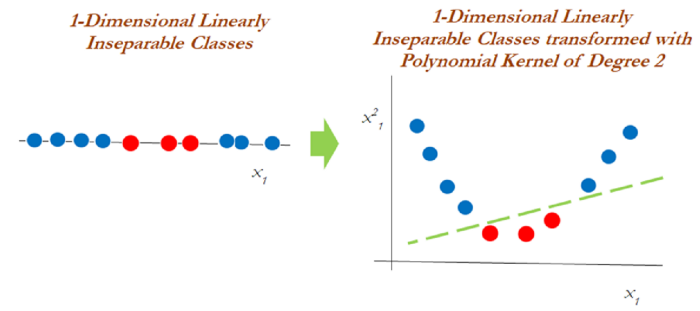
\includegraphics[scale=0.6]{../5-pictures/chapter-4-4_pic_17.png}
	\end{center}
\end{frame}
%..................................................................
\begin{frame}{The Kernel Trick}
	\begin{center}
	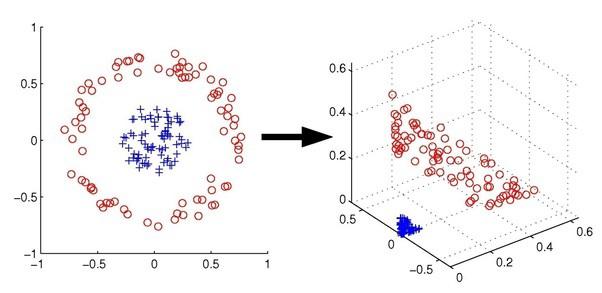
\includegraphics[scale=0.6]{../5-pictures/chapter-4-4_pic_18.png}
	\end{center}
\end{frame}
%..................................................................
\begin{frame}{Forming new features}
	\begin{itemize}
		\item We can add powers of each feature as a new feature.
		\item Alternatively, we can choose particular landmarks and create new features using the Gaussian Radial Basis Function (a similarity function). If values of features at a landmark are $l_1, l_2, \dots, l_m$, the new feature values are calculated as $$\exp\left(-\gamma \sum\limits_{j=1}^m (x_j - l_j)^2 \right)$$
		\item As the parameter $\gamma$ increases the span of influence of a landmark decreases  and the boundary becomes less smooth
	\end{itemize}
\end{frame}
%..................................................................
\begin{frame}{SVM Regression: using SVM to predict a continuous variable}
	\begin{itemize}
		\item We search for a pathway with a certain width that includes as many target values as possible
		\item If a target value lies within the pathway there is assumed to be no error
		\item If it lies outside the pathway the error is the difference between the actual value and the value predicted by the outer edge of the pathway 
	\end{itemize}
\end{frame}
%..................................................................
\begin{frame}{The single feature case}
	\begin{center}
	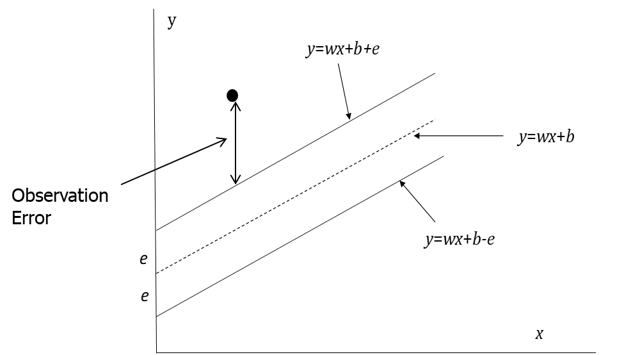
\includegraphics[scale=0.5]{../5-pictures/chapter-4-4_pic_19.png}
	\end{center}
\end{frame}
%..................................................................
\begin{frame}{General Case}
	\begin{itemize}
		\item We minimize $$C \sum\limits_{i=1}^n z_i + \sum\limits_{j=1}^m w_j^2$$   where $C$ is a hyperparameter
		\item $z_i$ is the error (zero if observation lies within the pathway)
		\item The first term is concerned with reducing errors for observations outside the pathway
		\item The second term provides some regularization. It avoids large positive and negative $w$s
	\end{itemize}
\end{frame}
%..................................................................
\begin{frame}{Example}
	Predicting Iowa House Prices from Living Area when e=50,000 and C=0.01 (Hull Figure 5.7)
	\begin{center}
	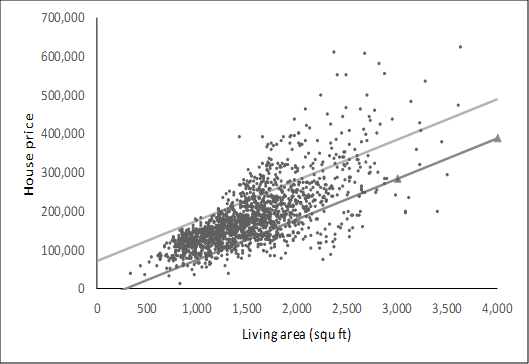
\includegraphics[scale=0.5]{../5-pictures/chapter-4-4_pic_20.png}
	\end{center}
\end{frame}
%..................................................................
\begin{frame}{Example}
	Predicting Iowa House Prices from Living Area when e=100,000 and C=0.1 (Hull Figure 5.8)
	\begin{center}
	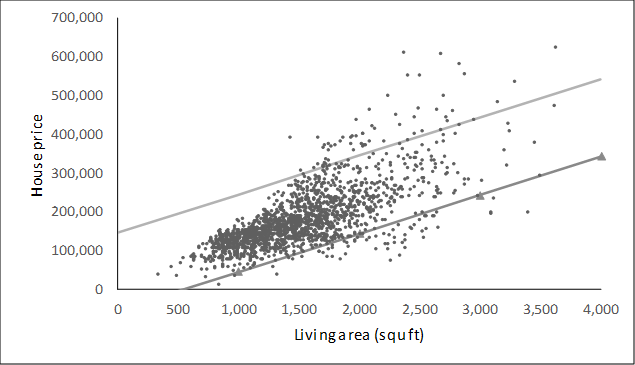
\includegraphics[scale=0.5]{../5-pictures/chapter-4-4_pic_21.png}
	\end{center}
\end{frame}
%..................................................................
%=====================================================================


\end{document}
